% As We May Think Software — versión en español
% Compila con pdflatex (arXiv) y con XeTeX/Tectonic.
\documentclass[11pt,a4paper]{article}

\usepackage{iftex}
\ifPDFTeX
  \usepackage[utf8]{inputenc}
  \usepackage[T1]{fontenc}
  \usepackage{mathpazo}
\else
  \usepackage{fontspec}
  \setmainfont{texgyrepagella}[Extension=.otf, UprightFont=*-regular, BoldFont=*-bold, ItalicFont=*-italic, BoldItalicFont=*-bolditalic]
\fi

\usepackage[spanish,es-noshorthands]{babel}
\usepackage{microtype}
\usepackage{graphicx}
\usepackage[margin=3cm]{geometry}
\usepackage[hidelinks]{hyperref}

\setcounter{secnumdepth}{0}

\newcommand{\separador}{\begin{center}* \quad * \quad *\end{center}}

\title{As We May Think Software\\[0.5em]
  {\large Actas apócrifas sobre una cultura de software alternativa}}
\author{Rafael Luque\\ {\normalsize OSOCO}}
\date{Enero de 2026}

\begin{document}

\maketitle

\begin{abstract}
Estas actas ficticias relatan la visita de un comité de ingenieros y
diseñadores de software a \emph{Atelier}, un taller de otra dimensión donde el
software no se escribe: se cura. Al otro lado del portal, el software se
entiende como un medio compartido para pensar: el comportamiento es el
material de diseño, las teorías del dominio se hacen visibles y discutibles,
la IA actúa como un colega que amplía el juicio en lugar de sustituirlo, y la
gobernanza es una propiedad legible del propio medio. El ensayo usa esta
ficción de diseño para preguntar no qué herramienta necesitamos, sino qué
medio necesitamos para pensar juntos.
\end{abstract}

\tableofcontents
\newpage

\section{El portal se abre}

La frase había quedado flotando en mi cabeza como lo hacen las últimas líneas
de un buen ensayo. No como conclusión, sino como invitación.

\begin{quote}\itshape
``If the physicists ever figure out how to control the portal, I would most
certainly want to come for a visit and see\ldots''~\cite{petricek}
\end{quote}

Durante meses, fue exactamente eso: una invitación literaria, una forma
elegante de dejar una puerta entreabierta.

Hasta que la puerta apareció.

Nos citaron en un hangar del norte de Londres. El tipo de espacio donde uno
espera encontrar cajas, herramientas y técnicos con chalecos reflectantes;
donde el aire huele a polvo y a electricidad; donde las cosas importantes
suelen parecer provisionales. Pero esa mañana, en el centro, había algo que no
encajaba con el resto del inventario: un vacío vertical, quieto y preciso,
como si alguien hubiera recortado el aire.

No tenía marco. No tenía pantalla. No emitía luz.

Simplemente estaba.

\begin{figure}[htbp]
  \centering
  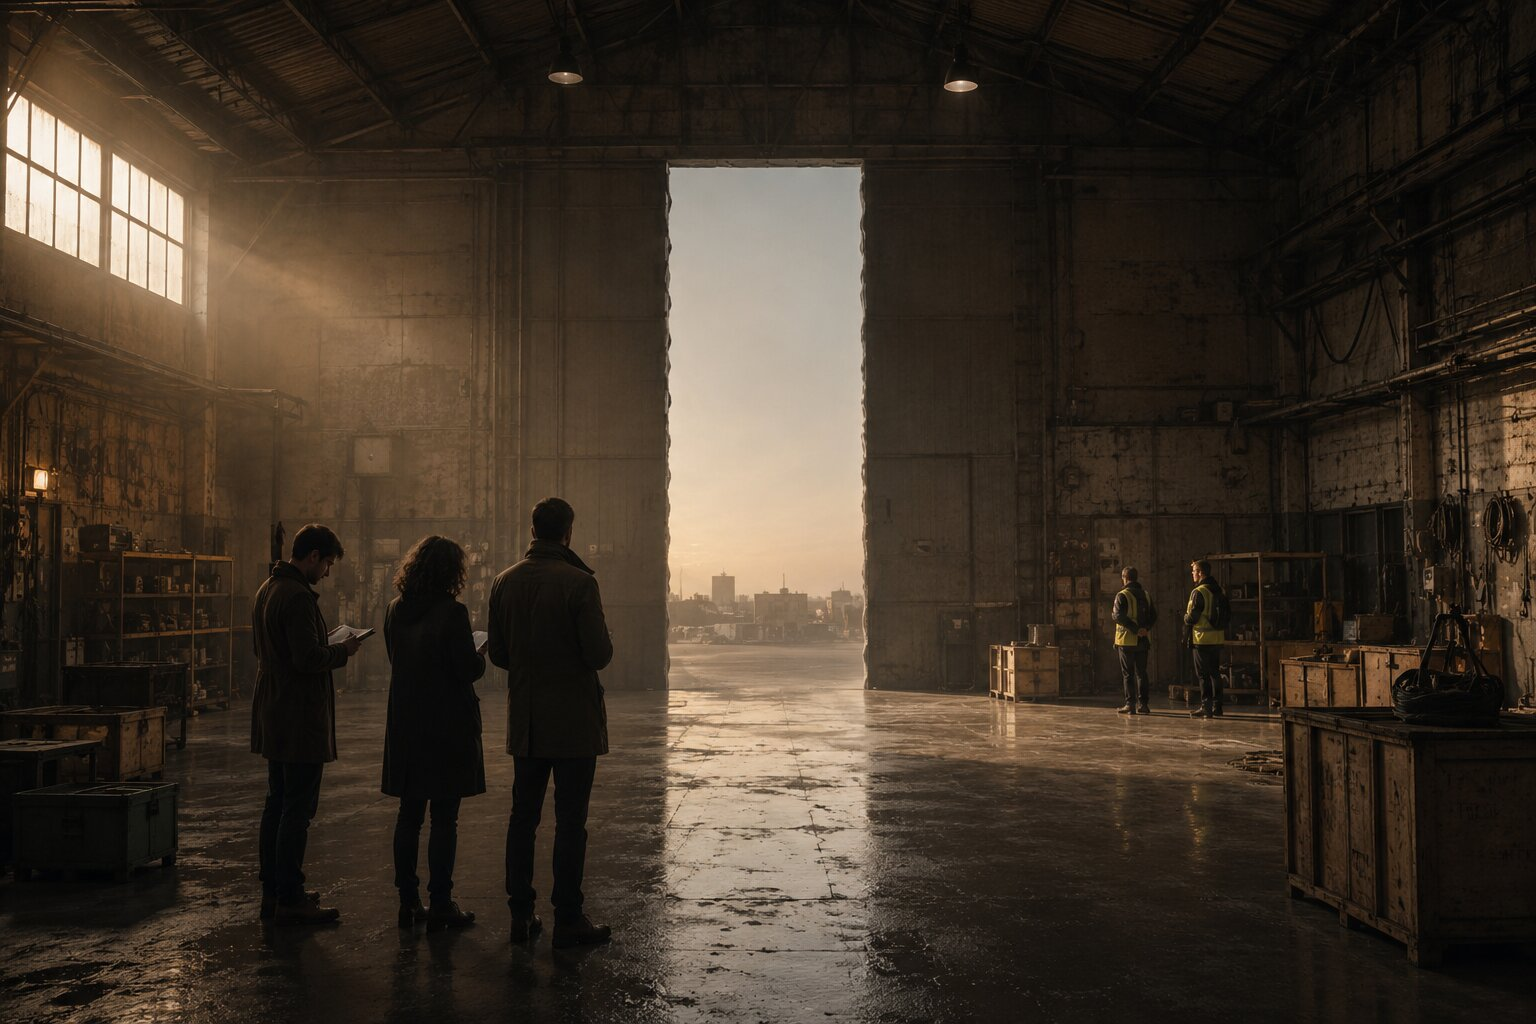
\includegraphics[width=0.85\linewidth]{figures/as-we-may-think-software-portal.jpg}
  \caption{El portal en el hangar: un vacío vertical, quieto y preciso.
    Imagen conceptual generada mediante IA.}
\end{figure}

Alrededor, un pequeño grupo de personas hablaba en voz baja, con esa mezcla de
nervios y profesionalidad que precede a las demostraciones que nadie se atreve
a llamar ``históricas''. Entre ellas estaba el comité que me habían pedido
acompañar. Un puñado de ingenieros y diseñadores de software reunidos para
observar y dejar constancia de lo que ocurriera al otro lado, si es que
ocurría algo.

Yo llevaba la libreta abierta antes incluso de saber qué iba a escribir.

Nadie pronunció ``inter-dimensional''. Nadie dijo ``portal'' en alto. Solo nos
entregaron una tarjeta blanca con unas breves instrucciones:

\begin{center}
\textbf{Cruzar. Observar. Tomar actas.}
\end{center}

Cuando el aire en el borde del hueco onduló ligeramente, como si alguien
acabara de activar algo, sentí que el hangar dejaba de ser un hangar y pasaba
a ser un umbral.

No era luz. No era sonido. Era esa clase de cambio que se nota sin saber
explicarlo: el vacío ya no parecía solo un vacío. Parecía una abertura.

Entonces crucé.

\subsection{Nota del narrador}

Escribo esto como acta y como confesión. Acta, porque el comité me pidió
precisión. Confesión, porque me di cuenta de que lo que yo llamaba
``desarrollo'' era, en parte, un pacto cultural: una forma de aceptar que el
software se hace en texto, en pantallas, en archivos; que los desacuerdos se
detectan tarde; que los usuarios son el final de una cadena.

En el otro lado, ese pacto no existía. En su lugar había otro.

\separador

\section{Llegada al taller}

La primera impresión, al cruzar, fue desconcertante: el espacio parecía estar
vivo.

El lugar no era un laboratorio. Era más bien un estudio de diseño o un taller
de algún tipo de artesanía.

Una pared entera era blanca, pero no era un lienzo pasivo: reaccionaba como lo
hacen las cosas cuando sirven para pensar. Las mesas eran enormes, como las
mesas de un taller de carpintería, y estaban llenas de objetos corrientes:
cajas de cartón, fichas de madera, un móvil viejo, una cinta métrica, un
ticket impreso. Había también herramientas que parecían de oficina
---rotuladores, tarjetas de papel, tijeras--- salvo por un detalle: cuando
alguien las tocaba, el espacio respondía con luz, texto y movimiento, como si
los objetos fueran parte del sistema nervioso de aquel lugar.

\begin{figure}[htbp]
  \centering
  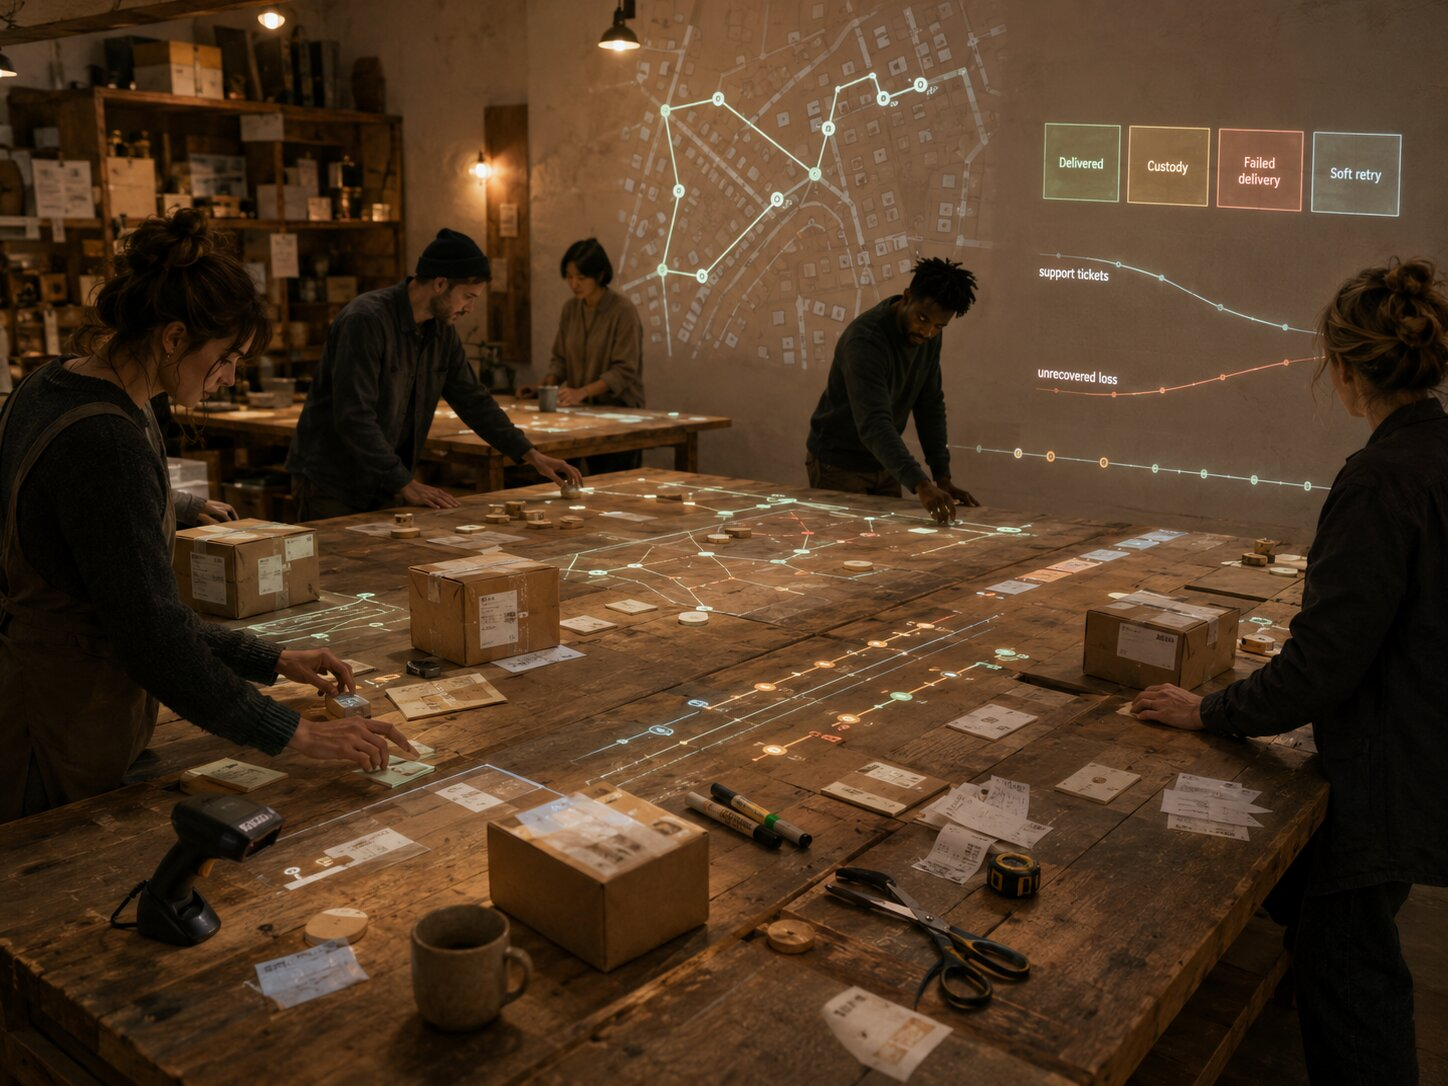
\includegraphics[width=0.85\linewidth]{figures/as-we-may-think-software-workshop.jpg}
  \caption{El taller de Atelier: mesas de carpintero y objetos cotidianos con
    capas digitales proyectadas. Imagen conceptual generada mediante IA.}
\end{figure}

Más tarde nos explicarían que aquello no era ``realidad aumentada'' en el
sentido de gafas y dispositivos personales, sino un tipo de computación
espacial que proyectaba información sobre superficies y dotaba de
comportamiento a materiales cotidianos, inspirada por ideas como las de
Dynamicland: un ``medio dinámico'' para que personas reales exploren ideas
juntas en el mundo real~\cite{victor}.

En nuestro mundo, la computación tiende a encogerse: ventanas dentro de
pantallas, pestañas dentro de esas ventanas, contexto en miniatura. Allí, la
computación se expandía hasta convertirse en el ambiente. No había que ``abrir
una herramienta''. Ya estabas dentro de ella.

Al otro lado nos esperaba una mujer con una sonrisa tranquila, como si recibir
comités interdimensionales fuese parte del trabajo de cualquier martes.

---Bienvenidos ---dijo---. Soy Adele Engelbart.

El apellido cayó en la sala como cae un nombre propio que ya contiene una
tesis. Vi cómo algunos miembros del comité se miraban, buscando el chiste.
Adele no les dejó tiempo.

---No es un homenaje ---aclaró---. Es una línea de trabajo. Si habéis venido
hasta aquí, ya intuís cuál: aumentar el intelecto humano~\cite{engelbart} sin
confundir ``aumento'' con ``automatización''. Aquí no venís a ver máquinas que
sustituyen. Venís a ver talleres que ayudan a pensar.

Nos condujo por un espacio amplio. No había filas de monitores. No había una
sala de ``ingenieros'' y otra de ``negocio''. Había mesas grandes y paredes
vacías, objetos cotidianos colocados con intención, y una luz que parecía la
de un estudio.

---A esto lo llamamos un \emph{ambiente de diseño} ---dijo ella---. Un medio
computacional compartido: el ordenador como taller.

Hizo una pausa, como quien decide si revelar o no un nombre propio.

---Y el nombre se nos quedó ---añadió---: \textbf{Atelier}.

---Antes de empezar ---dijo---, una advertencia: si intentáis traducir esto a
``un IDE en 3D'', os vais a perder. El cambio no es el decorado. Es el
material con el que se diseña.

Alguien del comité preguntó lo inevitable:

---¿Dónde está el código?

Adele señaló una pared vacía.

---Primero vais a ver un desacuerdo. Si al verlo pensáis ``esto es ciencia
ficción'', vamos bien. Esa sensación es el primer paso para desaprender lo que
hoy dais por natural.

\section{La pared pide la palabra}

En la mesa había un paquete real, de cartón, con una etiqueta a medio
despegar. A su lado, un rotulador, una libreta, un lector de códigos y una
taza de café que alguien había dejado demasiado cerca del borde. Nada parecía
``informática''. Y, sin embargo, lo era todo.

---Si lo marcamos como \emph{entregado} aquí ---dijo Alan, señalando el
paquete---, soporte deja de perseguirlo y el barrio deja de odiarnos.

---Soporte deja de perseguirlo ---repitió Vera--- ¿Y la persona que lo espera?

Alan iba a responder cuando la pared, literalmente la pared, pidió la palabra.

No fue un sonido de notificación. No fue una ventana emergente. Fue una frase
sobria, proyectada a la altura de los ojos sobre la pared blanca, como si
alguien hubiera escrito con tiza directamente sobre la pintura:

\begin{quote}
\centering
\textbf{``Hay dos definiciones incompatibles de `entregado' en esta sala.''}
\end{quote}

Debajo aparecieron dos tarjetas:

\begin{itemize}
  \item \textbf{Entregado (operaciones):} ``el caso se cierra; no requiere
    acción''.
  \item \textbf{Entregado (cliente):} ``el objeto está en manos del
    destinatario''.
\end{itemize}

\begin{figure}[htbp]
  \centering
  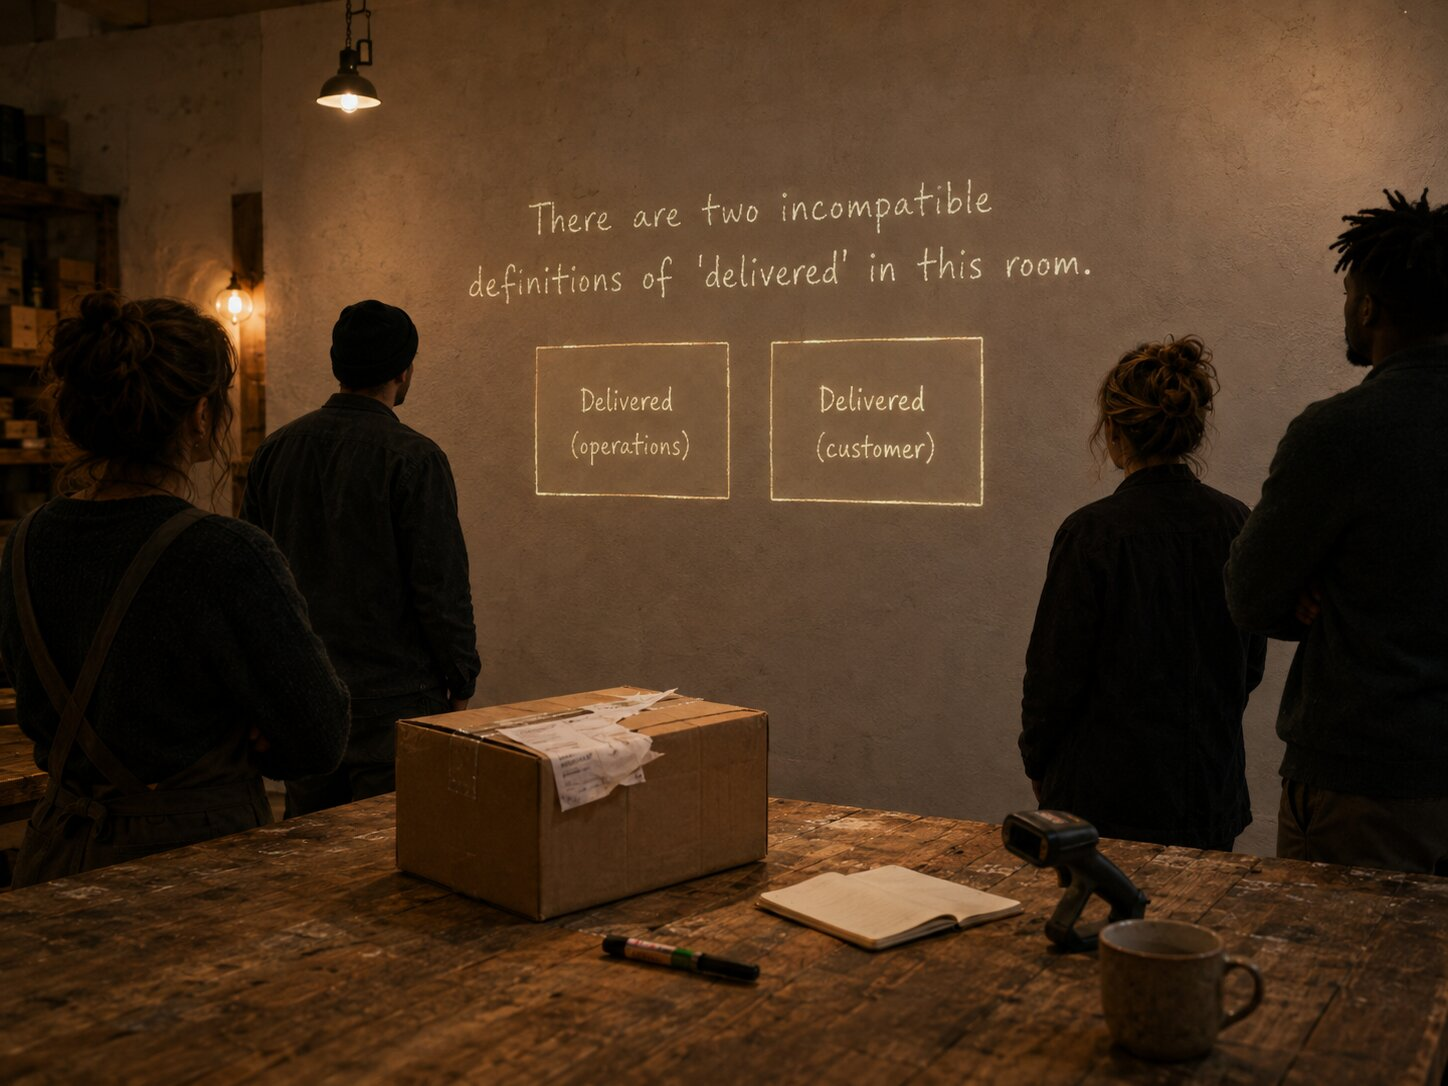
\includegraphics[width=0.85\linewidth]{figures/as-we-may-think-software-wall.jpg}
  \caption{La pared del taller hace visible el desacuerdo: dos definiciones
    incompatibles de ``entregado''. Imagen conceptual generada mediante IA.}
\end{figure}

Sentí algo extraño: el tipo de vergüenza que no viene de cometer un error,
sino de descubrir que llevabas años ignorando un error estructural. En mi
mundo, esas dos definiciones habrían coexistido sin hablarse. Una en tickets y
métricas; otra en llamadas de soporte y enfado. Aquí el sistema las había
obligado a mirarse a los ojos.

Vera no se movió hacia un teclado. Se movió hacia el paquete. Lo deslizó unos
centímetros sobre la mesa, como quien cambia una pieza de una maqueta. En la
superficie apareció una línea de tiempo: intentos, escaneos, llamadas,
reclamaciones. Cada evento se ramificaba en consecuencias visibles, no como un
diagrama estático, sino como una ejecución continua.

---Si decimos que ``escaneado en portal'' cuenta como entregado ---empezó
Vera.

La ejecución se adelantó a su frase. En el borde derecho de la mesa, una curva
subió: \emph{pérdida no recuperada en zonas de alto riesgo}. Otra bajó:
\emph{tickets de soporte}. La pared no celebró nada. No ``recomendó''. Solo
devolvió evidencia.

En un rincón apareció una nota breve, atribuida al agente de IA, con un tono
que me sorprendió por su modestia:

``Puedo mostrar tres escenarios históricos donde `escaneado en portal' se
correlaciona con pérdida. También puedo proponer un comportamiento alternativo
que mantenga la reducción de tickets sin cambiar el significado de
`entregado'. Si queréis, lo explico con ejemplos.''

Adele me miró ---o quizá miró al comité a través de mí--- y remató la escena
con una frase sin énfasis:

---¿Veis? Aquí el sistema interrumpe cuando el equipo usa una palabra para
nombrar dos mundos distintos. Ese es el ``ajá'' del taller. No la proyección,
sino lo que obliga a decir en voz alta.

La pared añadió una tercera línea:

\begin{quote}
\centering
\textbf{``Ambas teorías son válidas; el sistema no puede optimizar para las
dos sin introducir un estado intermedio.''}
\end{quote}

Apareció una palabra nueva: \textbf{``Custodia''}.

No fue un invento de la máquina. Fue el nombre que la conversación
necesitaba. El paquete no estaba ``entregado'' en el sentido humano, pero
tampoco ``pendiente'' en el sentido operativo: estaba accesible bajo
condiciones, con riesgo asociado, y ese riesgo era parte del contrato, no un
accidente.

Me sorprendí pensando que esto ---nombrar estados intermedios con
honestidad--- era exactamente lo que en mi mundo se pospone por prisa, hasta
que la realidad lo impone de la peor manera.

\section{El software como medio}

En la siguiente sala, Adele nos dio lo que en mi mundo habría sido ``la
presentación''. Aquí fue más bien una orientación, como la que te da alguien
antes de entrar en un taller de carpintería: no te habla de martillos, te
habla de madera.

---Atelier ---dijo--- parte de una cultura que entiende el software como
\textbf{medio} para pensar y crear. No como un subproducto del plan, sino como
un material epistemológico que sirve para razonar sobre un dominio, ensayar
hipótesis y construir comprensión.

Mientras hablaba, yo recordaba historias de otras épocas:
Smalltalk~\cite{ingalls} como un mundo, no como un lenguaje; la idea de un
medio dinámico personal~\cite{kay}; el aprendizaje por
construcción~\cite{constructionism}. Adele no lo mencionó como genealogía,
sino como evidencia de que otra relación con el ordenador siempre fue posible.

---Hoy ---continuó--- el software tiene un peso social y económico enorme. Si
es un medio tan poderoso, no basta con hacerlo rápido. Hay que hacerlo
comprensible, modificable y responsable. Y hay que hacerlo accesible a más
personas que ``los programadores''.

Alguien del comité preguntó si eso era una utopía.

Adele sonrió sin conceder demasiado.

---Es un oficio. Y como todo oficio, tiene un precio.

\section{Teoría distribuida}

Uno de los miembros del comité citó a Peter Naur, quizá para anclar lo raro en
algo familiar: \emph{programming as theory building}~\cite{naur}.

Adele asintió.

---Sí. Pero hoy en día hay un matiz: el software no es la teoría de una
persona. Es el resultado de teorías distribuidas: de cada miembro del equipo,
de las herramientas, de los documentos, de las métricas\ldots{} y de los
agentes de IA cuando participan.

Esa frase me golpeó porque describía una realidad que yo conocía, pero no
había articulado. En mi mundo decimos ``alineamiento'', ``visión'',
``conocimiento compartido''. Pero lo hacemos alrededor de herramientas que
fragmentan. Tickets por un lado, código por otro, diseño por otro, soporte por
otro. Y luego nos sorprende que la palabra ``entregado'' signifique cosas
distintas.

---Atelier ---dijo Adele--- es un intento de alinear esa cognición
distribuida~\cite{dcog}. No con un documento más, sino con un medio de trabajo
que haga visibles las teorías, que permita discutirlas y que las someta a
prueba continuamente.

\section{El ordenador como taller}

Si yo escribiera el taller como ``computación espacial'' y ``realidad
aumentada'' como descripción principal, estaría mintiendo por reducción. Lo
importante no era el efecto visual, sino el cambio de hábitos que el espacio
imponía.

En Atelier no había ``pantalla principal''. El taller era el ordenador: mesas
grandes, paredes, superficies donde objetos físicos cotidianos convivían con
capas digitales superpuestas. El dominio entraba en el espacio como materia
---paquetes, etiquetas, formularios, planos, citas, reglas, excepciones. Y el
software no aparecía como texto, sino como comportamiento que se podía señalar
y mover.

\begin{figure}[htbp]
  \centering
  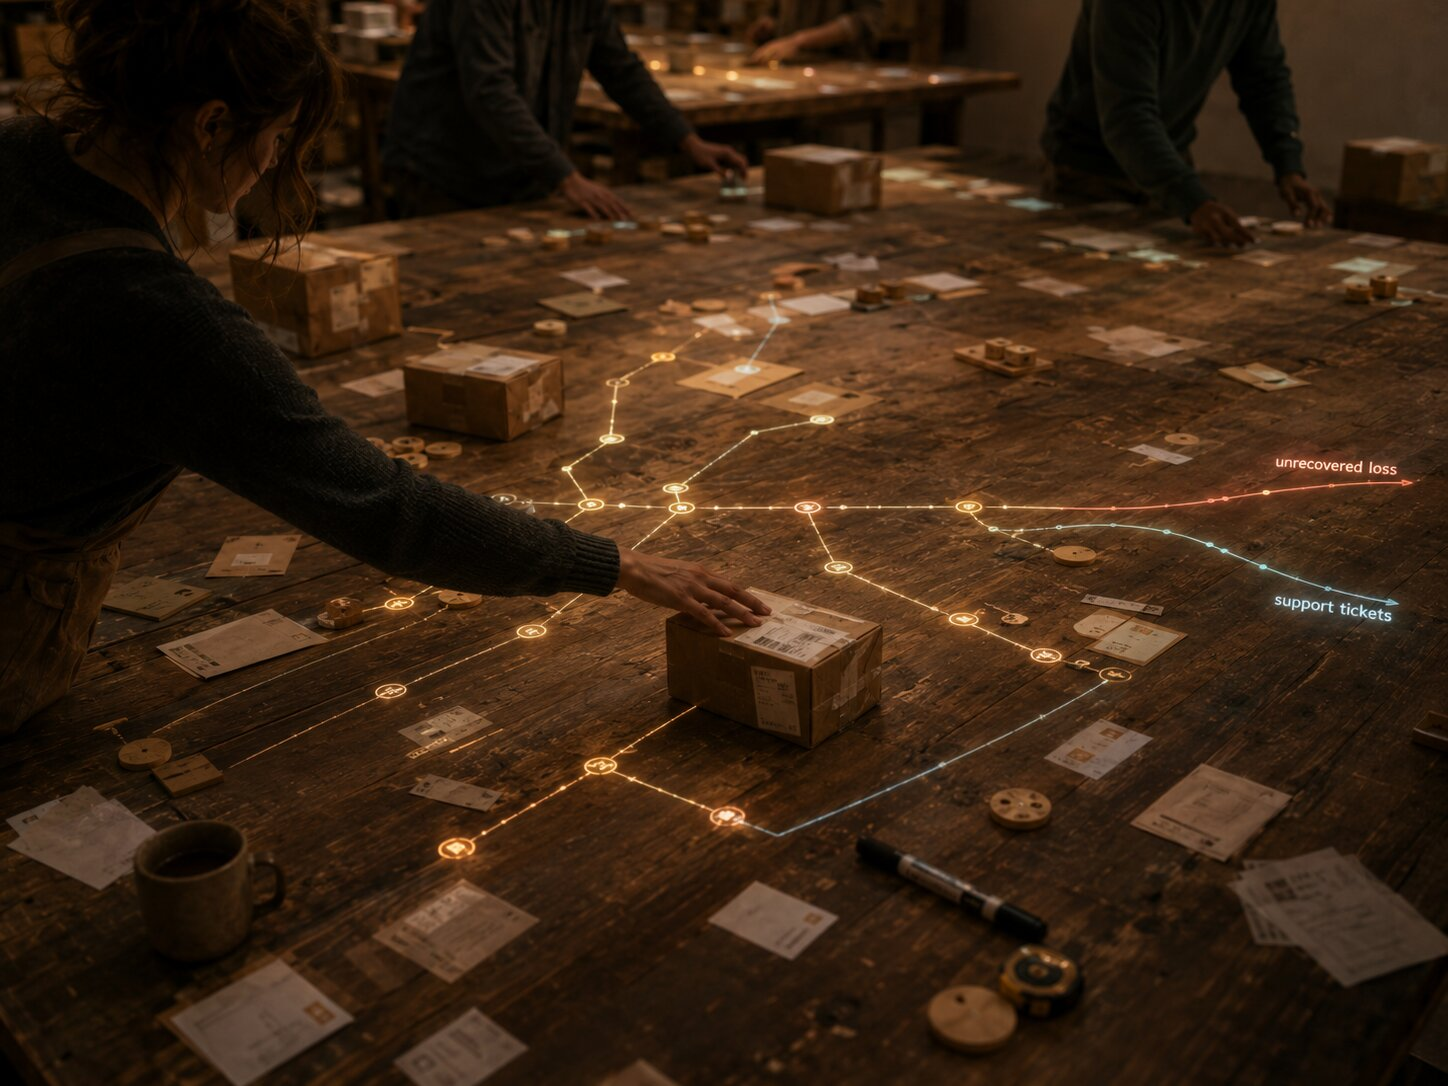
\includegraphics[width=0.85\linewidth]{figures/as-we-may-think-software-table.jpg}
  \caption{La mesa como superficie de simulación continua: el paquete real y
    sus consecuencias proyectadas. Imagen conceptual generada mediante IA.}
\end{figure}

Adele lo resumió con una frase que anoté literalmente:

---Aquí la interfaz no está hecha para escribir. Está hecha para negociar
significado con evidencia.

\section{Voces del taller}

Adele nos permitió hablar con algunas personas. Dijo ``personas'' con
intención. Ni ``roles'', ni ``recursos''. Aun así, cada voz encarnaba una
parte de la teoría.

\subsection{Vera ---curadora de comportamientos}

Vera me habló como si estuviera corrigiendo una confusión común entre los
visitantes.

---El cambio grande ---dijo--- es que dejamos de confundir ``programar'' con
``traducir''. Traducir a un lenguaje es útil, pero tiene un coste. Lo que no
cabe se vuelve implícito, y lo implícito es donde se esconden los desacuerdos.

Me señaló una zona de la pared donde había tarjetas de comportamiento. No eran
``funciones''. Eran frases con condiciones, excepciones y ejemplos.

---Nuestro material son descripciones legibles: ``cuando ocurra esto, entonces
aquello; excepto si\ldots''. Y cada comportamiento tiene ejemplos vivos. Por
debajo, sí, generamos sistemas ejecutables. Pero lo que curamos aquí no es
código bonito. Es coherencia de significado.

\subsection{Nico ---optimización con consecuencias}

---Yo fui el que metió la pata\ldots{} con la mejor intención.

---En el sistema antiguo, cada ``entrega fallida'' abría un circuito: se
avisaba a soporte, se programaba un reintento, se consideraba un punto de
recogida. En Atelier, el comportamiento estaba descrito de forma muy directa:

\begin{center}
\textbf{Si hay reintento y el mensajero confirma ``entregado'', cerramos el
caso.}
\end{center}

---Visto en la mesa, aquello me pareció demasiado ``caro'' para un problema
que yo veía cada día. Muchas alertas se disparaban por cosas pequeñas ---un
timbre roto, una puerta que no abre--- y eso saturaba al equipo. Así que
propuse un ajuste que, en mi cabeza, era de sentido común:

\begin{center}
\textbf{Si el paquete ha sido escaneado en el portal del edificio, lo
consideramos ``entregado'' y no iniciamos el circuito de reclamación.}
\end{center}

---En mi cabeza era eficiencia. En el taller fue un terremoto silencioso.

---Lo vimos al instante cuando arrastramos el escenario ``\emph{Barrio Sur ---
Semana 42}'' al centro de la mesa. La ejecución continua empezó a marcar como
``entregados'' paquetes que en realidad quedaban en el portal, donde se
pierden con frecuencia. Y como mi cambio cerraba el caso antes, ocurría algo
perverso. Había menos tickets, sí, porque el sistema dejaba de crear
reclamaciones\ldots{} pero también había menos investigación y menos
recuperación de paquetes realmente perdidos. El resultado no era solo ``menos
trabajo'', era más pérdida que ya no se intentaba recuperar, justo en los
barrios donde esa pérdida golpea más.

---Ahí entendí lo que me costó ver al principio: lo peor no fue el número. Fue
la palabra.

---Yo había cambiado el significado de ``entregado'' sin darme cuenta. Para
mí, ``entregado'' empezó a significar ``esto ya no requiere acción interna''.
Para la persona que espera el paquete, ``entregado'' significa ``lo tengo en
la mano''.

---La sala nos lo devolvió como contradicción visible: dos definiciones
incompatibles. Y eso te obliga a hacer algo que en el desarrollo tradicional
solemos posponer: declarar el contrato.

---Así que no ``revertimos código''. Ajustamos un contrato: ``entregado'' dejó
de ser un único sí/no y pasó a ser un \textbf{estado} que exige evidencia
suficiente. Y ``escaneado en portal'' dejó de cerrar el caso: se convirtió en
una señal que \textbf{propone} una hipótesis (``probablemente está ahí''),
pero que en zonas de riesgo exige confirmación adicional antes de afirmar que
está ``entregado''.

---Me gusta contarlo así porque cambia el tipo de vergüenza. No es ``programé
mal''. Es ``entendí mal''. Confundí una mejora para el equipo con una verdad
para el mundo.

\subsection{Alan ---historias y excepciones}

Alan, a quien yo habría llamado ``stakeholder'' en mi mundo, se rió cuando se
lo mencioné.

---Antes yo ``especificaba requisitos'' ---dijo--- y luego discutía con
fantasmas: ``yo no pedí esto'', ``esto no era así''. Aquí no doy requisitos.
Traigo casos, excepciones\ldots{} historias. Y el taller me devuelve
consecuencias.

Me di cuenta de que esa frase describía una redistribución de poder. El
dominio ya no tenía que traducirse para participar.

---Y no tengo que convertirme en programador ---añadió---. Tampoco tengo que
resignarme a ser ``usuario final''. Soy parte de la teoría.

\section{La IA como colega}

En Atelier, la IA no se comportaba como un botón de ``solución''. Se
comportaba más bien como una persona muy rápida procesando datos y patrones,
pero obligada ---por cultura y por diseño--- a jugar con reglas humanas:
explicar, sugerir alternativas, preguntar por supuestos, recordar decisiones,
señalar contradicciones.

No estaba al servicio de la delegación de nuestra inteligencia. Estaba al
servicio de la teoría compartida: de hacer visible lo que solemos dejar
implícito y de ampliar el espacio donde podemos razonar juntos sin convertir
el taller en una caja negra.

Lo vi con claridad en una discusión aparentemente banal sobre qué significaba
``inmediato''. Alguien lo dijo como quien dice ``rápido'' ---una palabra
elástica, cómoda, peligrosa. La IA no respondió con una definición única.
Respondió con un abanico.

---Puedo proponer tres definiciones de ``inmediato'' ---dijo---. Y, para cada
una, puedo mostrar dos cosas: qué mejora y a quién perjudica.

En la pared, junto al escenario activo, aparecieron tres formulaciones. No
``recomendaciones'', sino contratos posibles. Debajo de cada una,
consecuencias: menos fricción aquí, más fallos allá; más autonomía para este
grupo, más carga para aquel; mejor métrica, peor experiencia.

---No puedo decidir por vosotros ---añadió--- porque vuestra teoría del
dominio también incluye valores, no solo objetivos.

No supe si aquella frase era una convicción cultural o una restricción de
diseño. En ambos casos, funcionaba porque devolvía el juicio al equipo, pero
con más claridad, más opciones y más evidencia.

Más tarde, cuando se lo comenté a Adele, lo resumió con una frase que anoté
para mi informe:

---La IA aquí no reemplaza el juicio; simplemente amplía el espacio donde el
juicio puede ejercerse.

\section{Comportamiento antes que lenguaje}

En algún momento pregunté por el lenguaje.

---¿En qué lo escribís?

Adele me miró con una resignación paciente, como si hubiera oído esa pregunta
multitud de veces.

---Esa pregunta asume que nuestro trabajo es traducir una intención humana a
un lenguaje aceptable por la máquina ---dijo---. Aquí el trabajo es describir
comportamientos del modo más directo posible, de forma que puedan coexistir,
entrar en conflicto, resolverse y ejecutarse.

Señaló la mesa donde seguían viviendo, a la vista, las tarjetas de
``Custodia'', ``Reintento suave'', ``Entrega fallida'' y otras tantas. No eran
nombres de funciones. Eran piezas de un argumento.

---Lo importante es la representación ---continuó---. El comportamiento como
material de diseño: visible, discutible, ensayable, compartible y, por último,
ejecutable.

Me explicó que, por debajo, podían generar sistemas ejecutables usando un
paradigma cercano a lo que en nuestro mundo se conoce como \emph{behavioral
programming}~\cite{harel}: una forma de construir sistemas reactivos a partir
de especificaciones de comportamiento que se sincronizan y se componen.

Pero insistió en que esa capa ``de debajo'' no era el centro del medio. Lo
relevante era lo que la sala hacía posible: reducir el intervalo entre lo que
creemos estar diciendo y lo que el sistema realmente hará.

---Cuando diseñas así ---dijo---, el feedback deja de ser una fase que llega
días o semanas después. Se obtiene mientras la conversación está ocurriendo.

Hizo una pausa, no dramática, sino ética.

---Si el software es importante socioeconómicamente ---añadió--- y además es
un medio creativo, entonces no puede quedar encerrado en una gramática que
solo una subcultura domina. Tiene que ser estudiable, modificable y
remezclable por cualquiera.

Lo dijo sin épica. Como si fuera una obviedad que en nuestro mundo habíamos
olvidado.

\section{Accesibilidad sin ``usuarios finales''}

Adele fue explícita en una frase que el comité discutió durante horas:

---El software debería ser abierto y accesible para estudio y modificación por
cualquier persona. Sin distinciones entre programadores y usuarios finales.

Yo esperaba que alguien replicara aludiendo a la ``seguridad'',
``complejidad'', ``responsabilidad'', etc. Finalmente, lo hicieron y Adele no
negó nada de eso.

---Precisamente por eso el taller necesita legibilidad, trazabilidad y
guardarraíles ---dijo---. La accesibilidad no es ``todo vale''. Es ``todo
puede leerse'' y ``todo cambio debe poder justificarse ante quienes lo
sufren''.

Era una postura política sobre la alfabetización, pero presentada como una
exigencia de diseño.

\section{Gobernanza visible}

La última sesión con el comité fue la más tensa. Un miembro dijo algo que sonó
razonable incluso en el otro mundo:

---Si cualquiera puede tocar, ¿quién responde?

Adele se apoyó en la mesa como quien acepta el peso real de la pregunta.

---Abrir no elimina responsabilidad. La hace visible.

En Atelier, la gobernanza no era un documento externo. Era parte del material:
contratos de comportamiento con ámbitos claros, registros legibles de cambios
y motivaciones, simulaciones obligatorias para cambios de alto impacto,
límites por consecuencias y no por jerarquías simbólicas.

Adele dijo una frase que anoté porque me pareció el tipo de norma que mi mundo
intenta y rara vez logra:

---Si no se puede explicar, no se despliega.

No era una promesa moral. Era una condición de legibilidad.

\section{Epílogo: la pregunta correcta}

En la última parte de la visita, Adele nos llevó a una pared donde había
escrito algo que no era exactamente documentación ni decoración. Era un
manifiesto, pero escrito como se escriben las influencias en una escuela de
arte: para recordar a tu mano de qué tradición viene cuando trabaja.

En la pared habían dejado cuatro líneas sencillas:

\begin{itemize}
  \item Herramientas como mundos (no como utilidades).
  \item Computación como medio de pensamiento.
  \item Aprendizaje como construcción.
  \item Programación como teoría distribuida.
\end{itemize}

\begin{figure}[htbp]
  \centering
  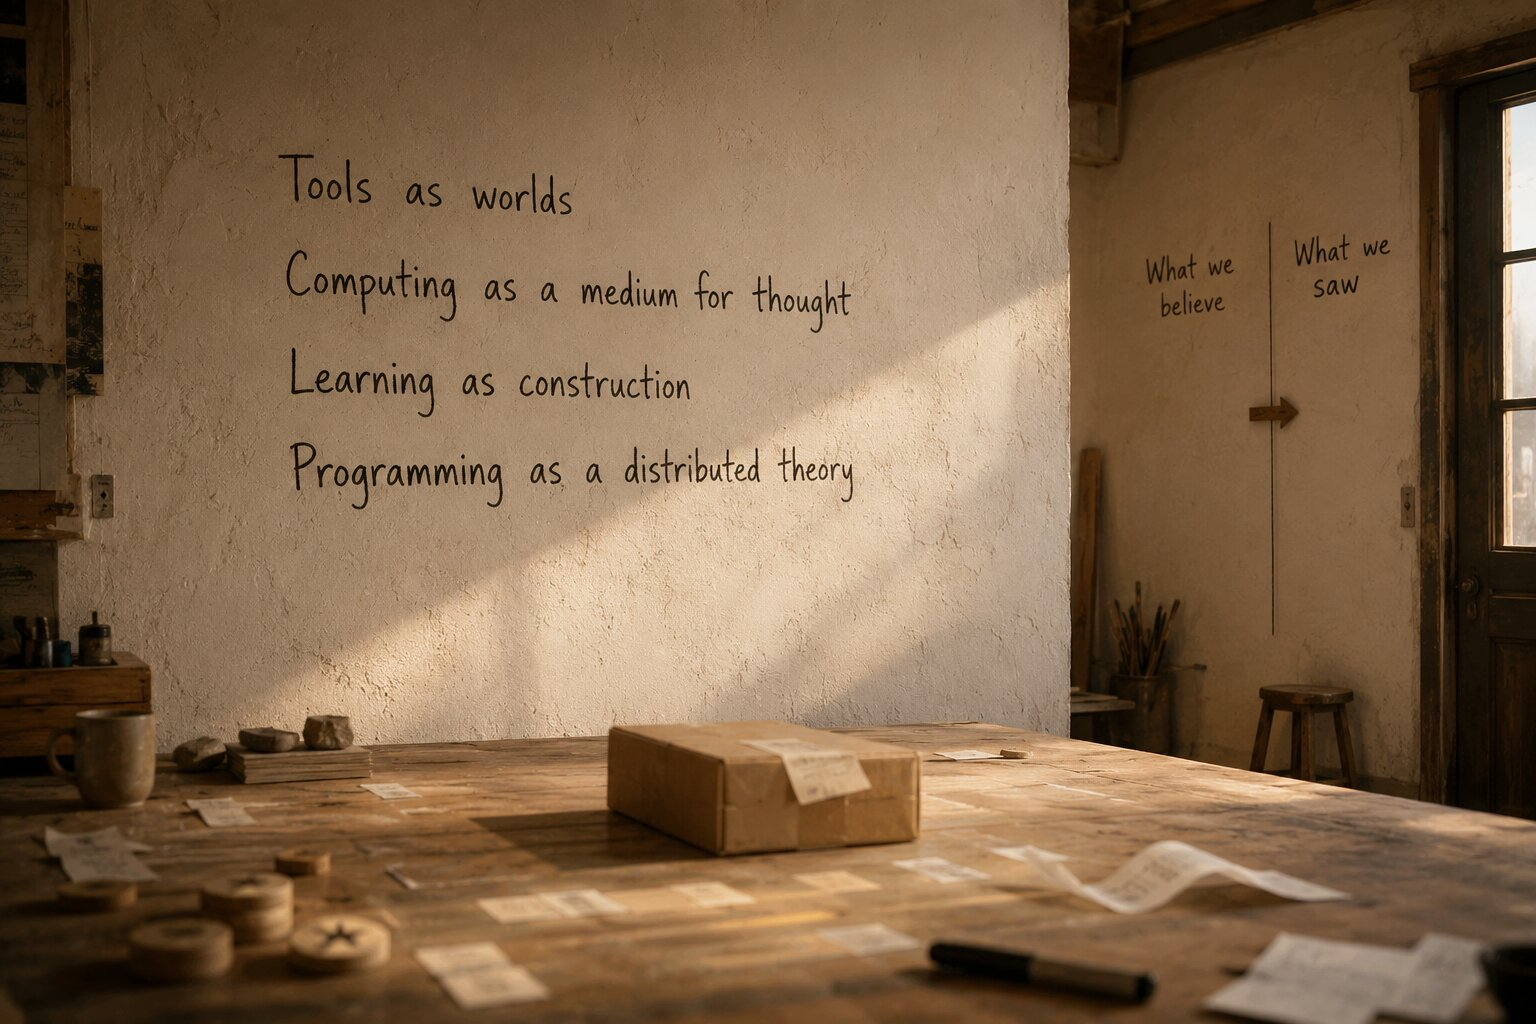
\includegraphics[width=0.85\linewidth]{figures/as-we-may-think-software-manifesto.jpg}
  \caption{El manifiesto del taller y las dos columnas ``Lo que creemos'' /
    ``Lo que vimos''. Imagen conceptual generada mediante IA.}
\end{figure}

No mencionaron nombres para impresionar. Pero el aire olía a esa tradición. La
idea de que el ordenador no es una máquina de escribir mejorada, sino un medio
que puede cambiar la forma en que razonamos; la idea de que aprender es
construir modelos con los que pensar; la idea de que el software puede ser un
material social.

Me quedé mirando esas líneas y, por primera vez en la visita, entendí algo con
una claridad incómoda. Atelier no era una herramienta ``para programadores''.
Era un taller donde la distinción entre programador y usuario final no tenía
sentido como frontera moral. Tenía sentido, si acaso, como diferencia de
práctica, como diferencia de familiaridad, pero en ningún caso como derecho de
acceso al sistema.

Entonces capté la idea diferencial. No era que el software ``se hiciera sin
código''. Era que el software se hiciera sin esa distancia ritual entre
quienes pueden tocar el comportamiento y quienes solo pueden padecerlo.

Antes de despedirnos, Adele señaló otra pared, más cerca de la salida. Allí
habían escrito dos listas a mano, casi como una costumbre del lugar:

\begin{center}
\textbf{Lo que creemos} \hspace{3em} \textbf{Lo que vimos}
\end{center}

Eran las dos columnas que usaban para trabajar. Su teoría explícita a un lado,
la evidencia del sistema ejecutándose al otro.

Entre ambas, una flecha imantada que cambiaba de sitio durante el trabajo. A
veces señalaba lo que el equipo estaba suponiendo, a veces lo que acababan de
observar. Era su manera de recordar que allí el progreso era un vaivén, no una
declaración.

---En vuestro mundo llamáis ``ingeniería'' a construir bajo incertidumbre
---dijo Adele---. Aquí intentamos nombrar algo más simple: mantener visible lo
que creemos y someterlo, una y otra vez, a lo que vemos, hasta que la teoría
aguante el contacto con el mundo.

De regreso, en el hangar, alguien preguntó ---con una excitación que me
pareció adolescente y sabia a la vez--- qué habíamos aprendido.

Yo quise responder con arquitectura, con paradigmas, con referencias
conocidas. Quise hablar de computación espacial, de composición de
comportamientos, de ciclos de feedback. Pero lo más honesto era otra cosa.

Aprendimos que nuestra industria ha aceptado un acuerdo erróneo: que el
software es demasiado importante para dejarlo en manos de cualquiera y, al
mismo tiempo, demasiado complejo para hacerlo comprensible para cualquiera.

En Atelier ese acuerdo se rompe desde el medio. El taller hace visible la
teoría, el comportamiento, las consecuencias. Y al hacerlo cambia el tipo de
conversación que un equipo puede tener: ya no discute solo sobre
implementaciones, sino sobre significados; no solo sobre velocidad, sino sobre
justicia del impacto; no solo sobre ``qué funciona'', sino sobre ``qué mundo
estamos afirmando cuando funciona''.

No sé si podemos construir Atelier mañana en nuestro mundo. Probablemente no,
o no del todo. Pero sí sé que podemos empezar a construir hacia ese mundo
haciéndonos las preguntas correctas.

En vez de ``¿qué herramienta necesitamos?'', ``¿qué medio necesitamos para
pensar juntos?''.

Y quizá esa pregunta sea el principio de un futuro donde diseñar software se
parezca menos a traducir instrucciones y más a construir y compartir una
comprensión.

\begin{thebibliography}{9}

\bibitem{petricek}
T.~Petricek.
\emph{Software designers, not engineers: An interview from alternative
universe}. Blog de Tomas Petricek, 2021.
\url{https://tomasp.net/blog/2021/software-designers/}

\bibitem{victor}
B.~Victor et~al.
\emph{Dynamicland}.
\url{https://dynamicland.org/}

\bibitem{engelbart}
D.~C. Engelbart.
\emph{Augmenting Human Intellect: A Conceptual Framework}.
SRI Summary Report AFOSR-3223, 1962.

\bibitem{ingalls}
D.~Ingalls.
``Design Principles Behind Smalltalk''.
\emph{BYTE Magazine}, agosto de 1981.

\bibitem{kay}
A.~Kay.
``Personal Dynamic Media''.
\emph{IEEE Computer}, 10(3):31--41, 1977.

\bibitem{constructionism}
\emph{Constructionism (learning theory)}. Wikipedia.
\url{https://en.wikipedia.org/wiki/Constructionism_(learning_theory)}

\bibitem{naur}
P.~Naur.
``Programming as Theory Building''.
\emph{Microprocessing and Microprogramming}, 15(5):253--261, 1985.

\bibitem{dcog}
\emph{Distributed cognition}. Wikipedia.
\url{https://en.wikipedia.org/wiki/Distributed_cognition}

\bibitem{harel}
D.~Harel, A.~Marron y G.~Weiss.
``Behavioral Programming''.
\emph{Communications of the ACM}, 55(7):90--100, 2012.

\end{thebibliography}

\end{document}
